\documentclass{article}

\usepackage{subfig}
\usepackage{float}
\usepackage{graphicx}
\usepackage{algorithm}
\usepackage{algpseudocode}
\usepackage{changepage}


\begin{document}
\begin{titlepage}
	
	
	\begin{center}
		\vspace{2 cm}
		{\Large \textsc{Simone Quadrelli} }
	\end{center}
	
	
	\begin{figure}[H]
		\vspace{2 cm}
		\centering
		
\includegraphics[width=0.30\linewidth]{tesiSCIENZE_TECNOLOGIE.jpg}
		
	\end{figure}
	
	\begin{center}
		\vspace{2 cm}
		{\Large \textsc{Machine learning project} }
	\end{center}

	\par
	\vspace{3 cm}
	
	\begin{center}
		{\large Academic year 2018 - 2019}
	\end{center}
\end{titlepage}

 \pagenumbering{gobble}
\newpage 
\pagenumbering{roman}
\tableofcontents
\listoftables
\listoffigures
\newpage

\pagenumbering{arabic}


\section{Introduction}
short abstract: what are your going to present in the report \\
statement of the problem/goal of the analysis and description of the data set(s) \\
list of three to five findings/keypoints \\
the analysis with wise commentary  \\
(optional) theoretical background of the used methods \\
conclusions (should include the findings/keypoints) \\
the Appendix, containing all the R code \\

The present project addresses the fruit and vegetable multiclass classification problem. Its objective of this project is to classify a variety of fruits and vegetables whose images are stored in a recently released dataset.\\
\\
Fruit and vegetable classification is a challenging task, there are two different kind of problems that must be overcome: vegetables and fruits within the same class can differ in shape and colour due to maturity and growth. On the countrary, vegetables and fruits in different classes, such as red apples or grapes, may be very similar both in textures and in colours. 
Fruit and vegetable classification has a key role in many industries: it can be exploited to make agriculter more autonomous than ever before in history, but it can also be applied to all stages of the supply chain to assess the quality of the products from the producer to the consumer. 
The ability of harvesting robots can be enhanced by enforcing fruit and vegetables recognition, indeed it may allow them to recognize not only the type of fruit or vegetable but also its maturity or wheter it is rotten. Moreover, autonomous classification provides more consistent quality assessment since it does not depend of the opinion of different workers.
\\\\
The projects will analyze the classification performance of three machine learning algorithms on different fruits. The k-nearest neighbour (knn) algorithm was used to compute a baseline, a more sophistocated, the support vector machines (SVM) algorithm was later used for classification. The last approach was to construct a convolutional neural network becausethey are knoen to suit well the image classification. The are two different kind of features that were extracted to feed the algorithms: the grayscale and the rgb representation of the images.

The objective of the project are
\begin{itemize}
\item analyze the classification performance of the knn and svm using the grayscale on a variety of fruits
\item analyze the classification performance of the knn and svm using the grayscale on a variety of fruits
\item analyze the classification performance of the knn and svm using the rgb sacle on a variety of fruits
\item analyze the classification performance of the knn and svm using the rgb scale on a variety of fruits
\end{itemize}
Descrivere cosa si trova nelle sezioni successive

\section{Dataset and Features}
The analyzed dataset, known as \textit{Fruits 360}, was originally published in 2017  by Horea Muresan and Mihai Oltean to address fruit and vegetable classification \cite{dataset}. The existence of either too small datasets or too low-quality dataset was most compelling problem.  On the countrary, this dataset provides more that 70000 images of 114 different fruits and vegetables> Each image has a definition of 100 $\times$ 100 pixels. To increase the reliability of the results, it contains images of rotated fruits and vegetables. However those images make the training process much harder .
As the authors explain, the dataset was produced as follows: fruits and vegetables were planted in the shaft of a low speed motor (3 rpm) and a short movie of 20 seconds was recorded. However, due to the variations in the lighting conditions, the background was not uniform and a dedicated algorithm was exploited to extract the fruit from the background. The images were of such high quality that no preprocessing was required.
It is also worth noticing that the dataset was already splitted in train and test set, therefore no further splitting was required.\\
Fruits and vegetables have several distinct visual characteristics that can be extracted from the images. Colour, shape, size and texture are the most commonly used features\footnote{Features are the characteristics of an object that can distinguish it from other objects} in image classification.  Among all the possible feauters that can be extracted from an image, colours features play a key role in fruit and vegetable classification. Indeed, they seem to suit the domain and their computation is very fast and efficient \cite{review}. The project focuses on the grayscale and rgb representation of the images. \\
The following lines introduce the reader to some concept of colour spaces and colour representation.
Colour spaces are a specific organization of colors the allows to  reproduce the representation of colours. Two different colour spaces were exploited in this project: grayscale and the rgb.
\subsection{RGB colour space}
The RGB colour model is an additive color model, meaning that red, green and blue are added together to reproduce an wide array of colors. A color in the RGB colour model is described by indicating how much of the red, green, and blue is included. The colour of a pixel is expressed as an RGB triplet (R,G,G). Each component can vary from 0 to 255, since each channel is represented by a byte.


\subsection{Grayscale colour space}
Since the dataset contains rgb images, it was necessary to extraxt a grayscale representation of the pixels to be used as features.
In grayscale representation each pixel is a byte, meaning that the possible values it can be in range from 0 to 255. \\
The conversion algorithm implemented by the library \textit{imager} is the Luma algorithm. Each rgb channel $R, G, B$ of a pixel are passed to a function $\Gamma(x)$ to obtain its transformation, respectively $R', G', B'$. \\
The $\Gamma$ function is defined as: 
\begin{equation}
 x' = \Gamma(x) = Ax^{\gamma}
\end{equation}
where $x$ in the pixel intensity, $A$ is a scalar whose value is often $1$ and $\gamma$ is usually $\frac{1}{2.2}$.\\
To obtain the final grayscale representation  $y$ of a pixel $x$, the following linear transformation is applied  \cite{grayscaleconversion}
\begin{equation}
 y = 0.21 R' + 0.71 G' + 0.07  B'
\end{equation}


\section{Data analysis}
The procedure described in the following is the same for grayscale features and rgb features.
The first step in the analysis was the data extraction and the creation of the data matrix and the vector of the labels. 
The images have 100x100 pixels, but to limit the compuational complexity of the following algorithms i decided to resize them to 50x50 pixels.
The feature vector are extracted using the functions of the library \textit{imager}. Onche the data vectors are extracted , a data matrix is created. Each row of the matrix contains the linearized representation of the image. A separate vector of labels was create, one for each image. 

\begin{algorithm}[H] 
   \caption{Schema of the analysis}
    \begin{algorithmic}[1]
    \State Feature extraction
    \State Dimensionality reduction
    \State Extraction of the most significant features
    \State Construction of a baseline using knns
    \State Evaluation of svm
    \State CNN
\end{algorithmic}
\end{algorithm}

\noindent Most learning algorithms are exponentially slow in the number of the feature or at least significantly slow down as the number of feature increases. Furthermore, it is reasonable to belive that many of the pixels are useless since they are just part of the background. As a result i choose to reduce the dimensionality of the data using the Principal component analysis (PCA).  It is one of the most common technique to reduce the dimensionality of the data since it is very efficient. Once all the principal componenet are computed we can choose a subset of the that cna explain most of the variance.
\begin{figure}[H]  
  \begin{adjustwidth}{-4cm}{-4cm}
     \subfloat{%
       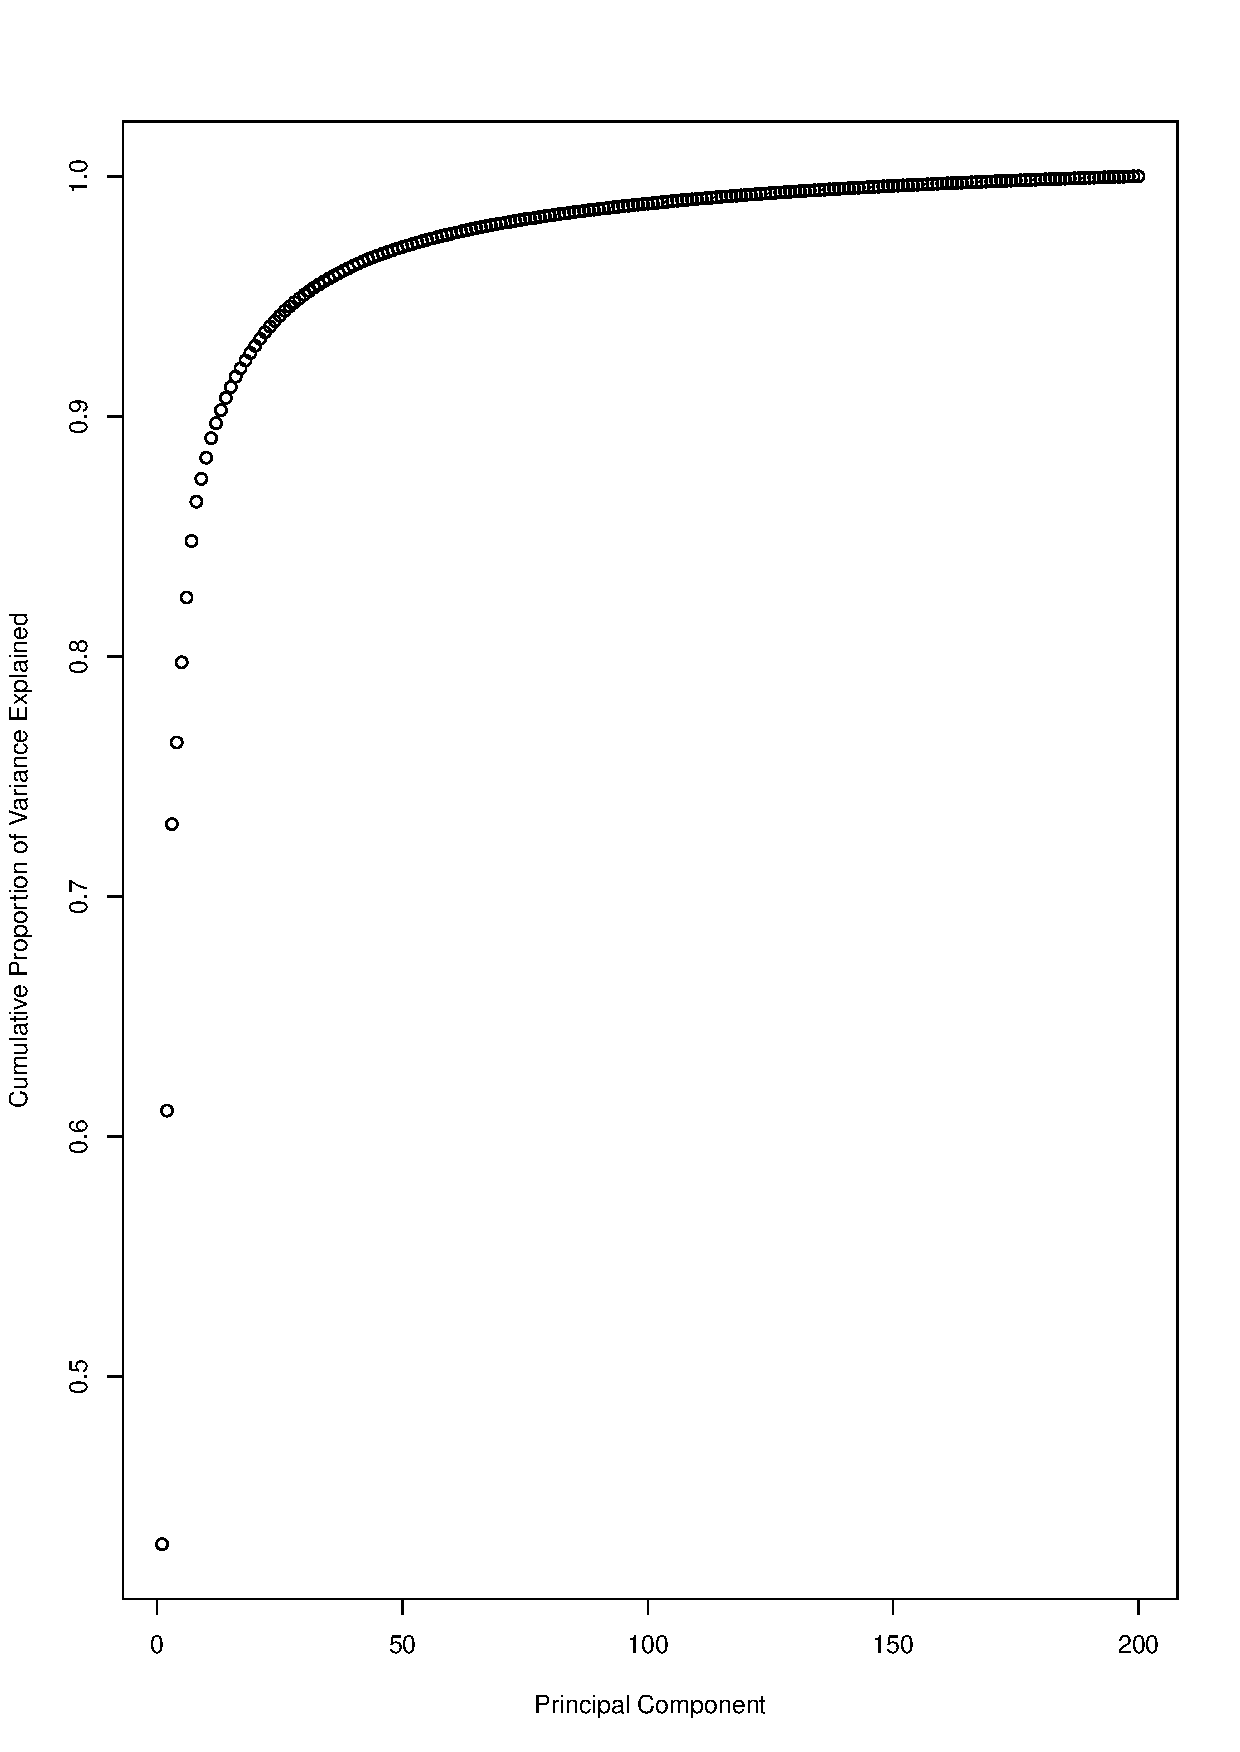
\includegraphics[scale=0.3]{../cumulative_variance_graysalce.pdf} 
     }
     \subfloat{%
    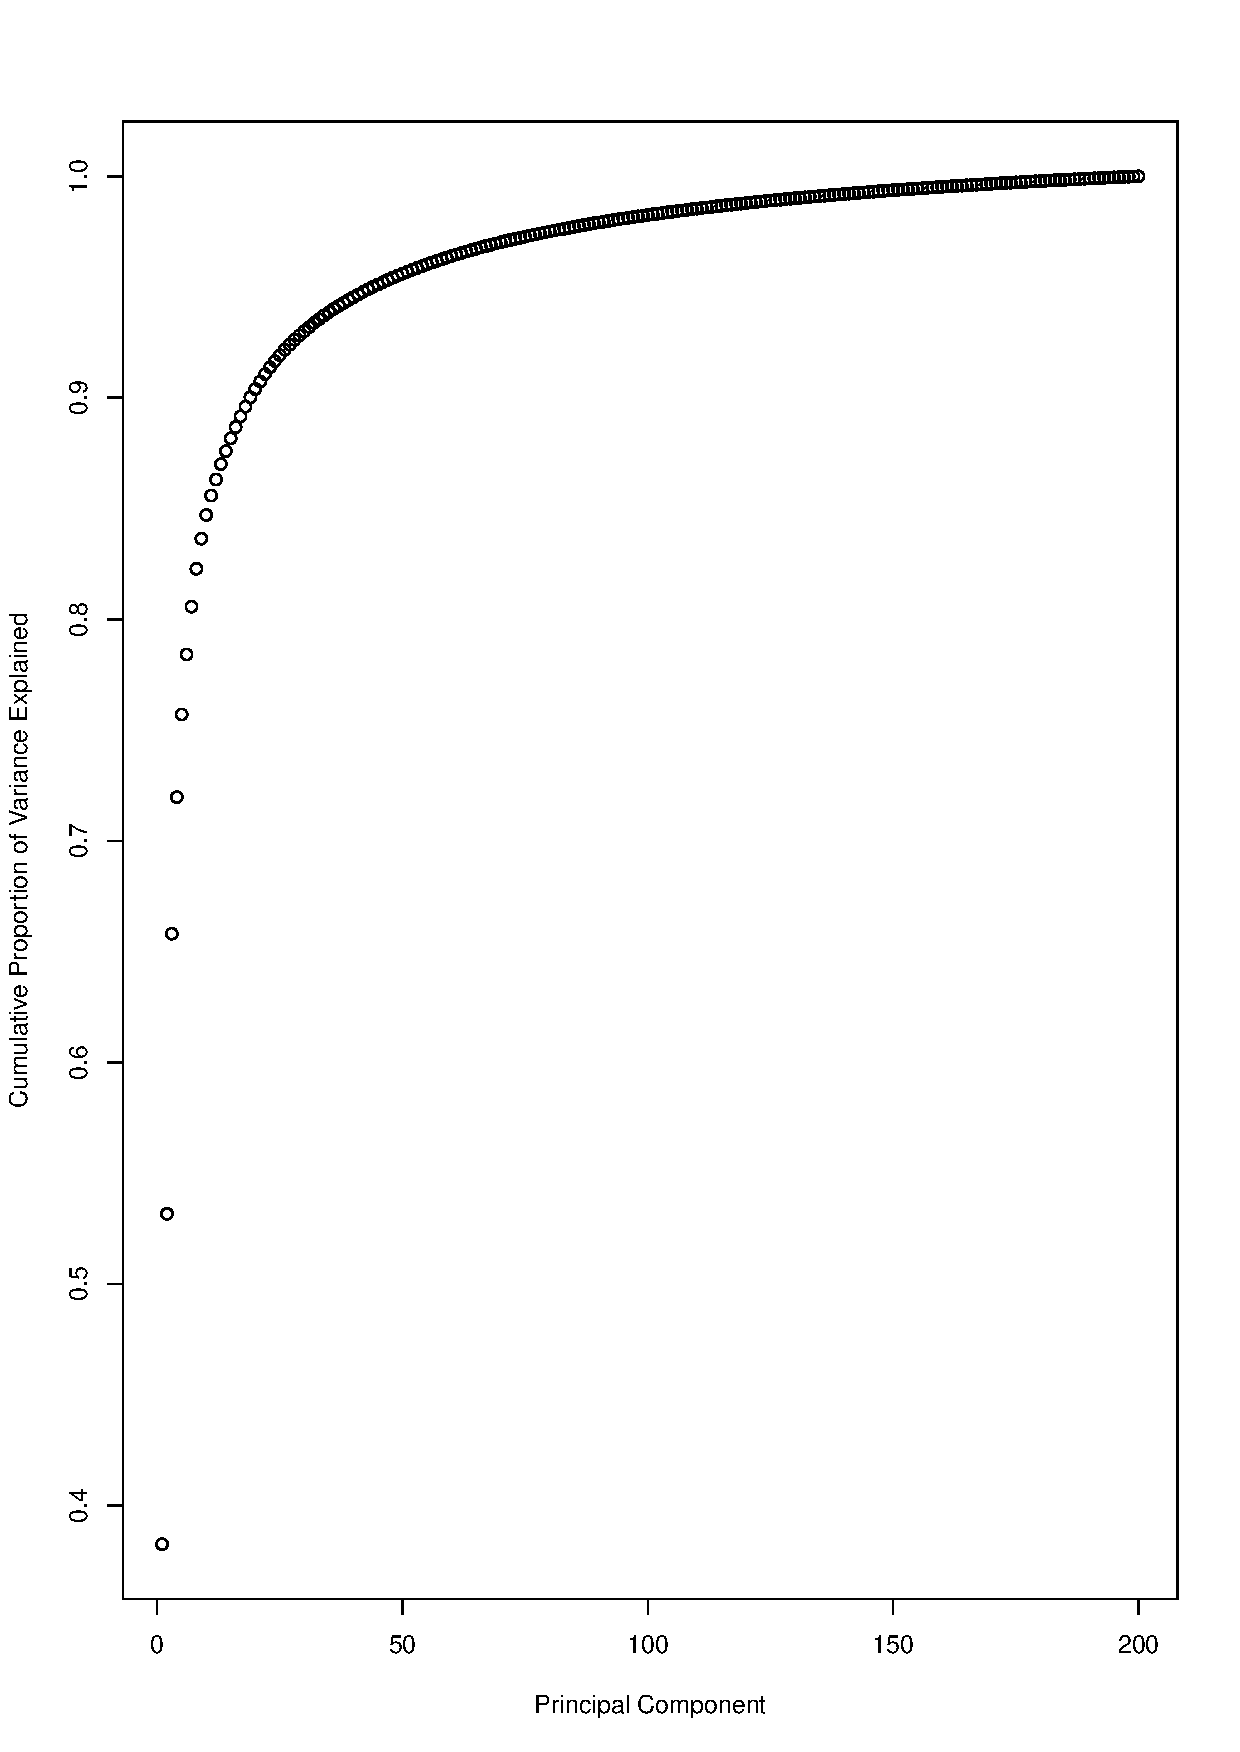
\includegraphics[scale=0.3]{../cumulative_variance_grb.pdf} 
     }
     \centering
     \caption{Cumulative variance}
      \end{adjustwidth}
   \end{figure}

\noindent As the plost above show, in both cases, using 150 is enough to explain all the variance in the data. However, having fixed the number of compunents, rgb components explain less variance than the grayscale components. To compare and analyze the performance of the learning algorithms i choose to use the following set of principal components $\{3,10,50,100,150\}$.  \\
\subsection{Baseline and knn}
The rationale behind this choice is to find the number of components that give the best result having at the same time a fast execution time. The k-nearest neighbours (knn) algorithm because it is known to be one of the most efficient classification algorithm even if it is very simple and dated \cite{knnresults}. Moreover, in image classification seem to perform quite as well as more sophisticated algorithms such as support vector machines. Bearing in mind  that, it seems to me the best choice to define a baseline. \\
As can be seen from the plots below there is no remarkable diffenrence in performace if the number of features considered in 10 or more. On the other hand, when only three features are uses the algorithms achieves lower performances. This difference is even more sharp when rgb features are involved, indeed its accuracy rate is about 0.10\% below the other accuracies. The best number of features to select is 50, since with all the possible value of k knn performs best with 50 features.\\
If we limit our analysis considering just the result of knn with at least 10 features 1-nn has the very best results, even if up to  4 neighbours there is no significant difference in performances.
Overall, knn reaches a very significant accuracy. The accuracy level  when considering rgb features reach up to 0.91.


\begin{figure}[H]  
  \begin{adjustwidth}{-4cm}{-4cm}
     \subfloat{%
       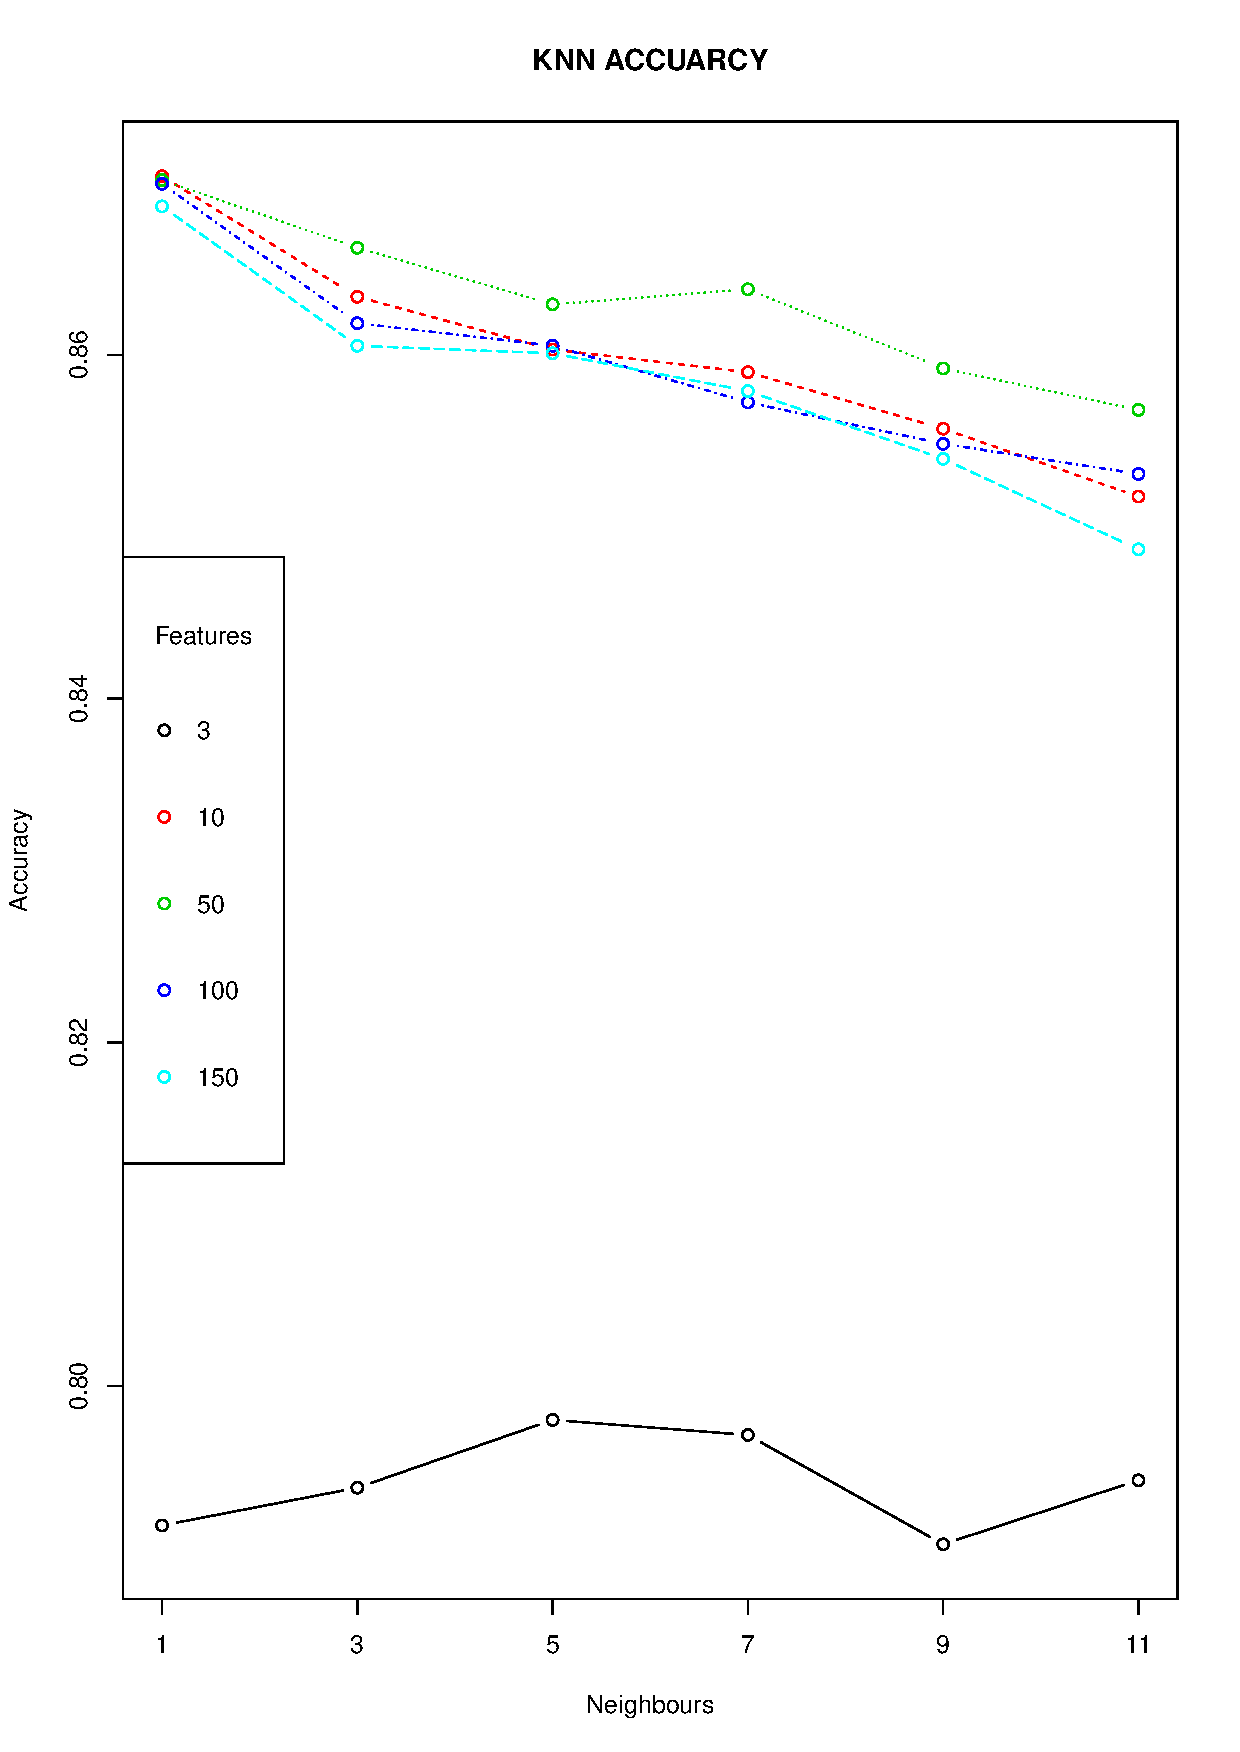
\includegraphics[scale=0.35]{../knn_accuracy_grayscale.pdf}
     }
     \subfloat{%
    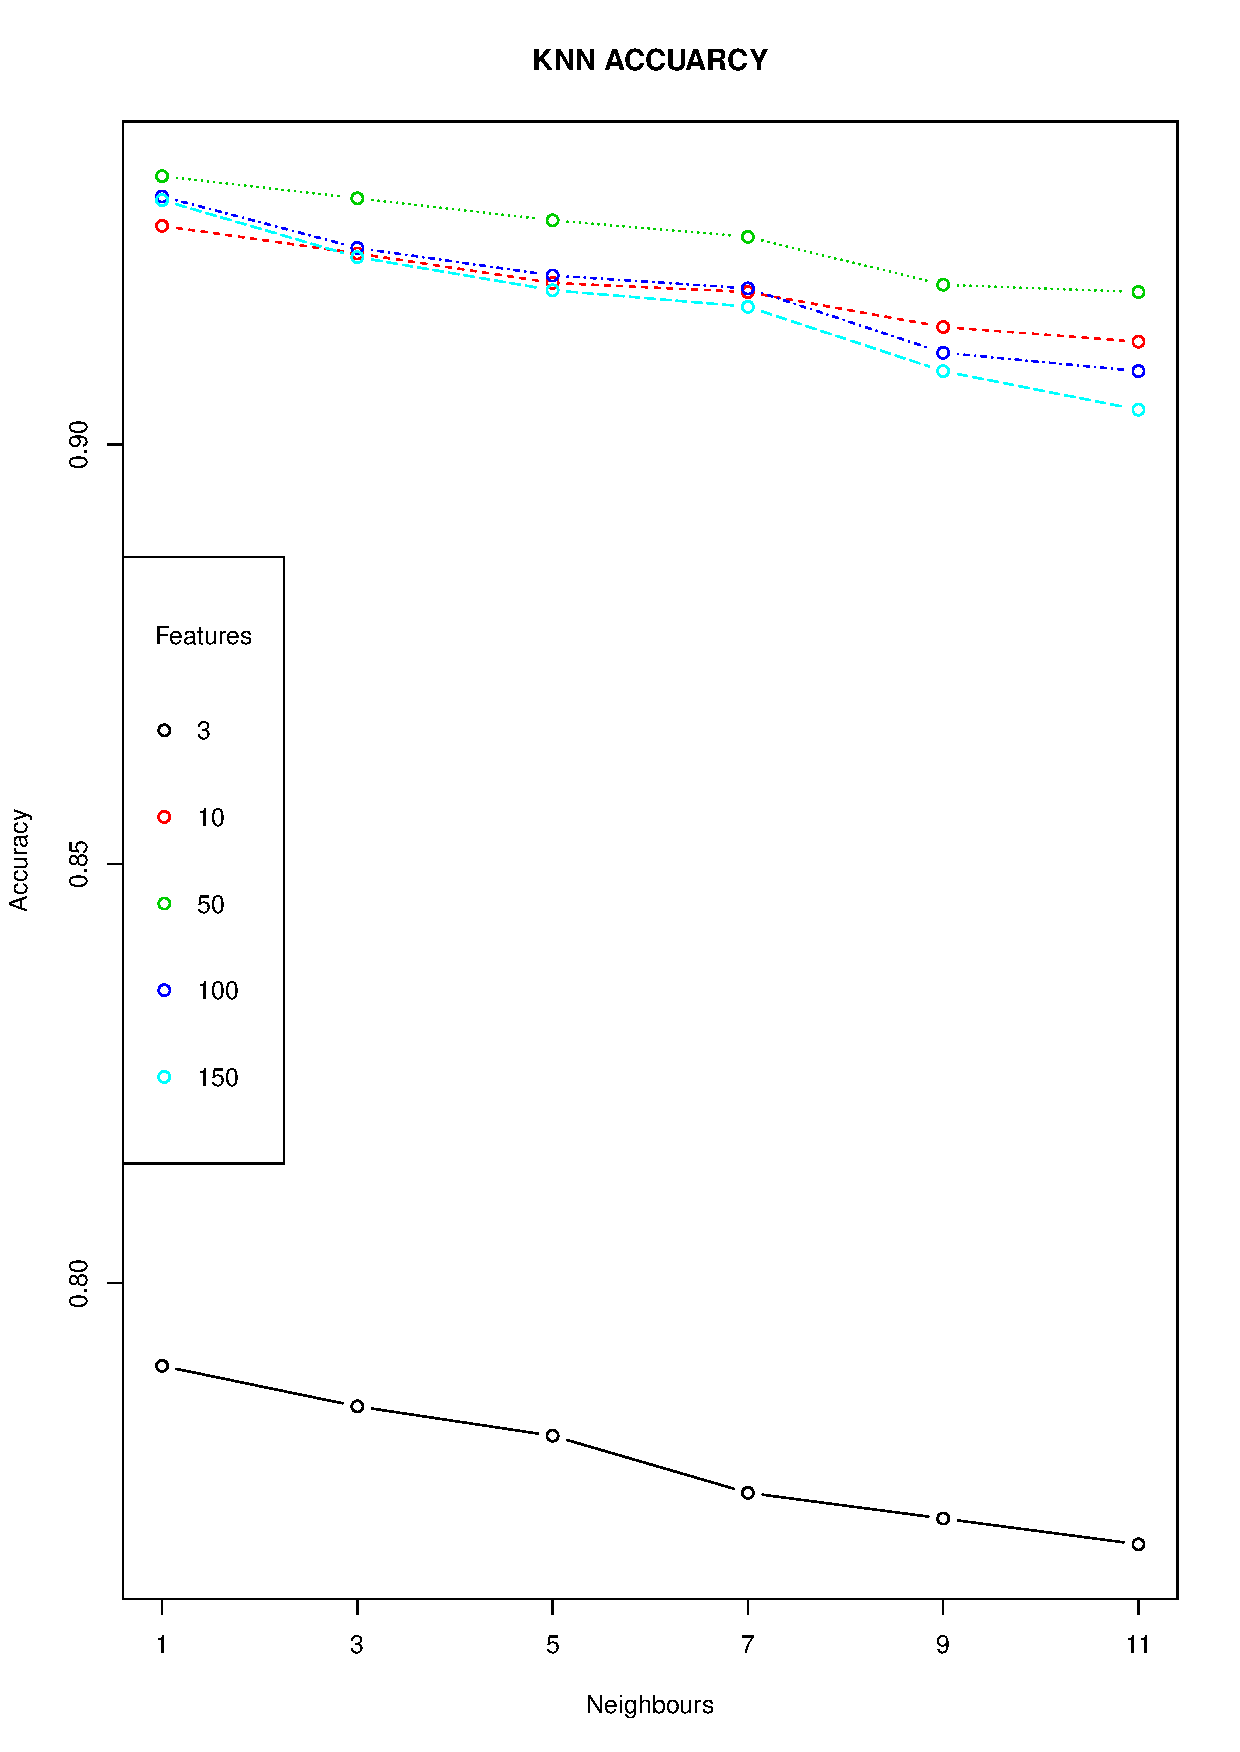
\includegraphics[scale=0.35]{../knn_accuracy_rgb.pdf}  
     }
     \centering
     \caption{Test performance knn}
      \end{adjustwidth}
   \end{figure}
\noindent The execution time of the algorithm is acceptable and does not exceed 30s. It is worth noting that the execution time, given the number of features, have just neglegible variation when the number of neighbours changes.\\
If one was to use just one model, I would recommend to choose a 1-nn with 50 features.


   
\begin{figure}[H]  
  \begin{adjustwidth}{-4cm}{-4cm}
     \subfloat{%
       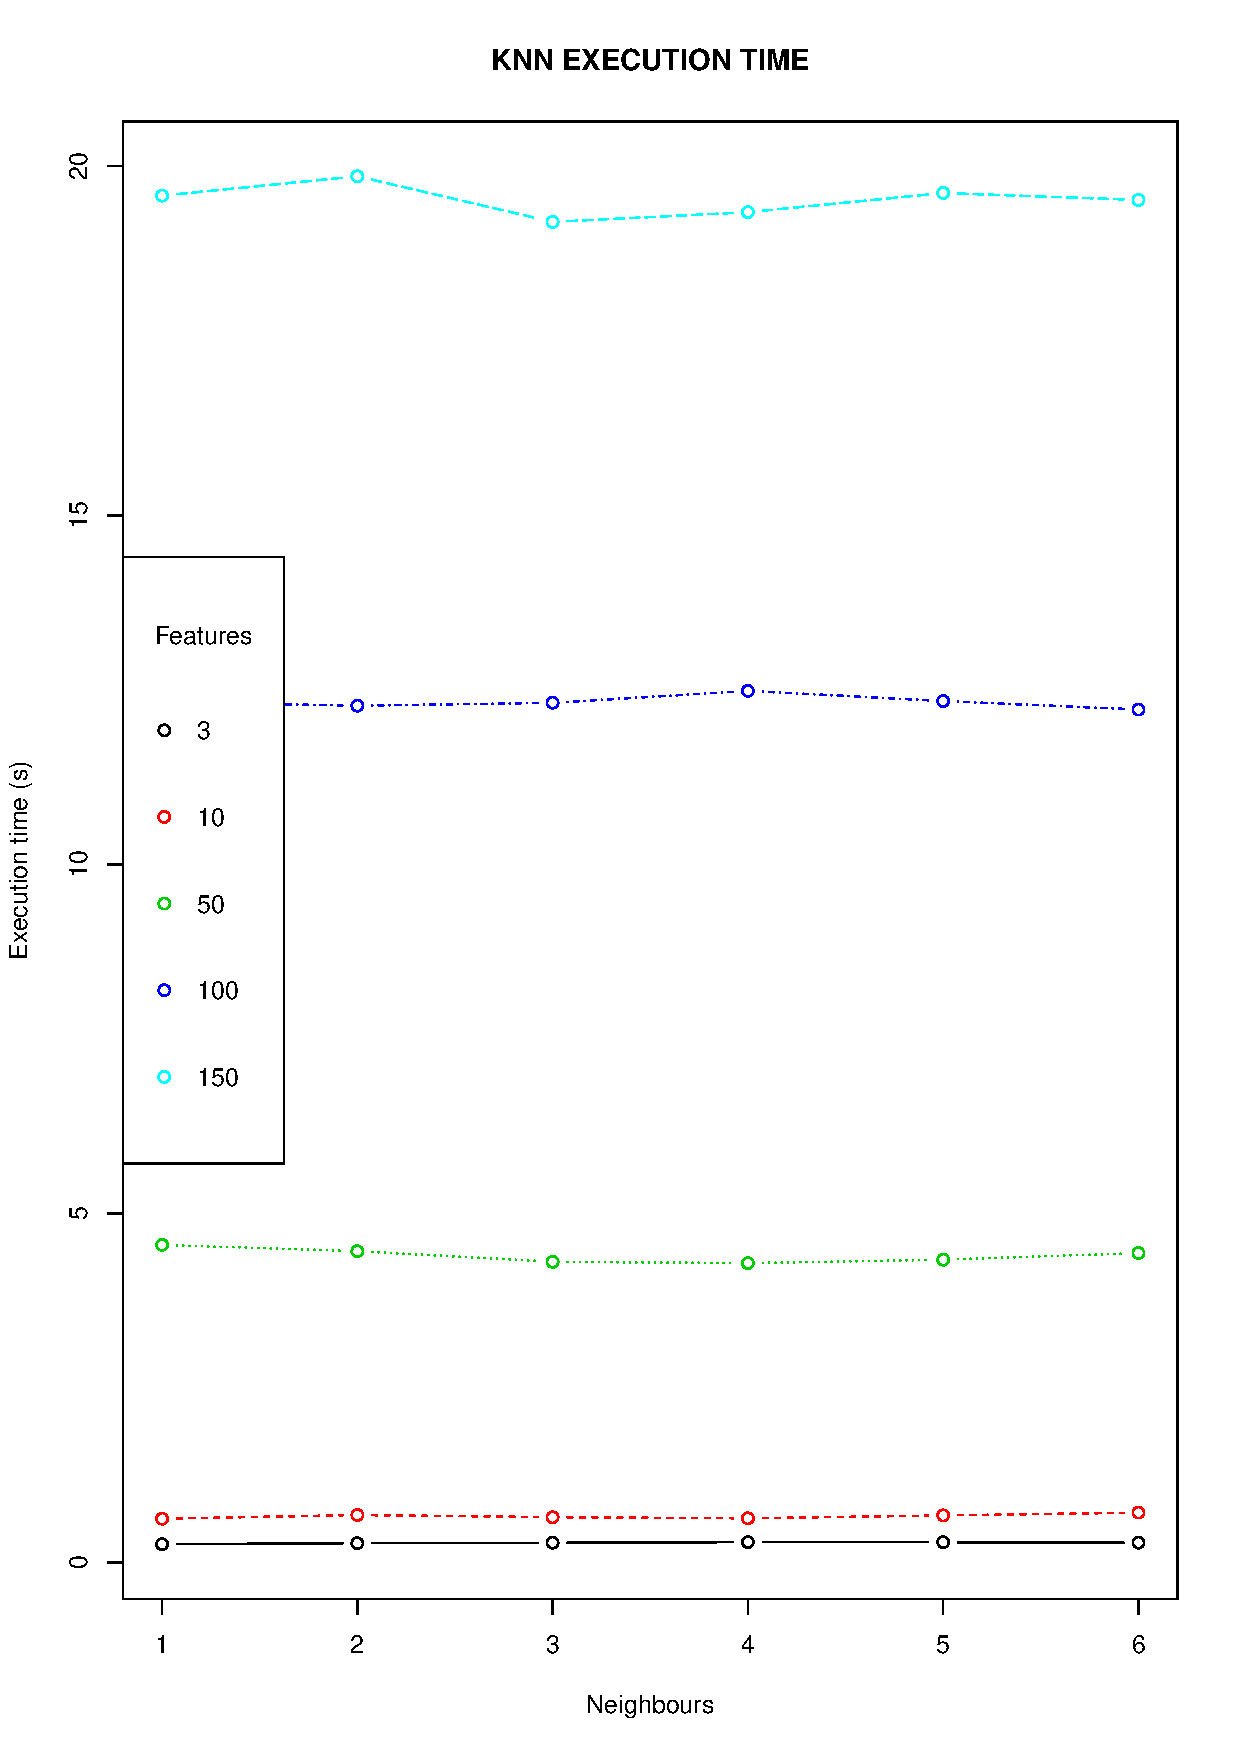
\includegraphics[scale=0.3]{../knn_time_grayscale.pdf}
     }
     \subfloat{%
    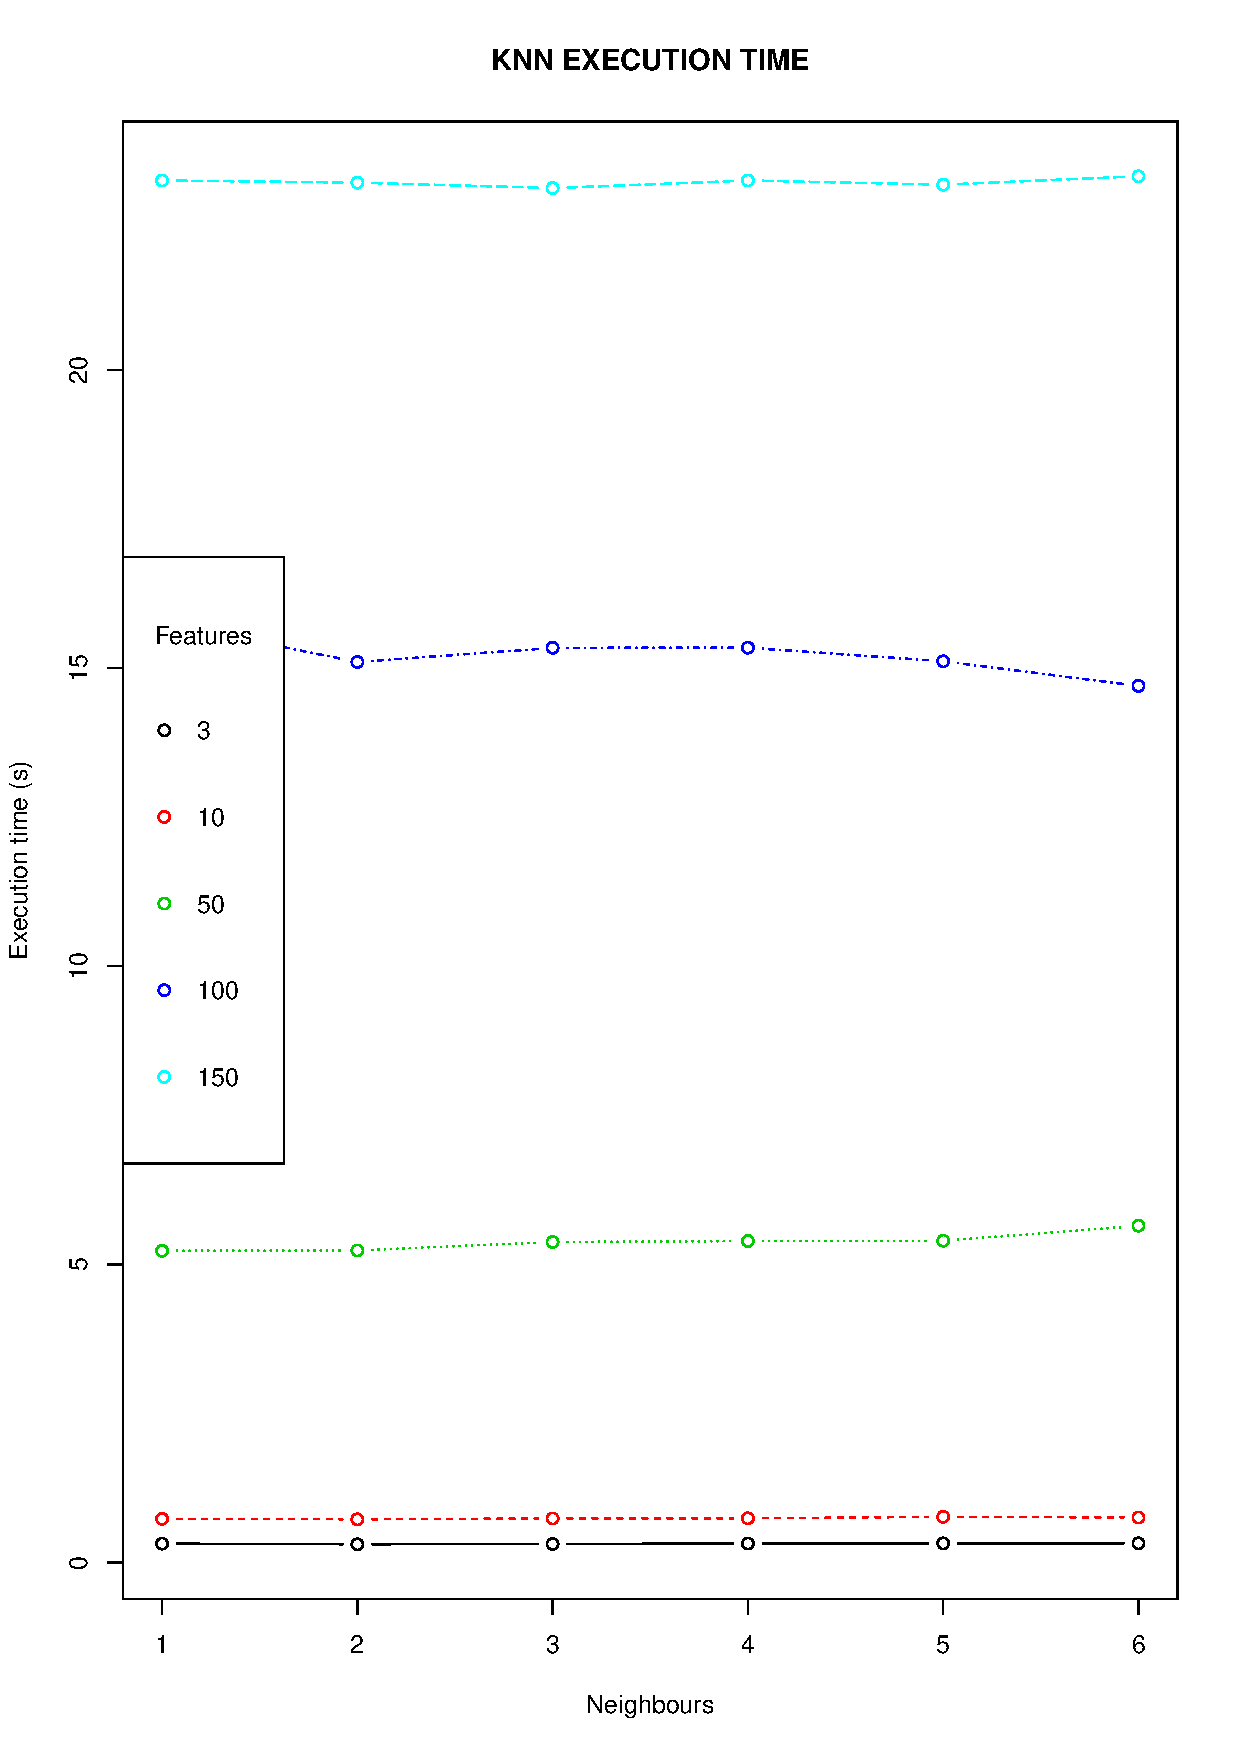
\includegraphics[scale=0.3]{../knn_time_rgb.pdf}  
     }
     \centering
     \caption{Execution time knn}
      \end{adjustwidth}
   \end{figure}

\subsection{SVM}
Support vector machines are often used in image classification. They are classification algorithm that provide 
\begin{figure}[H]  
  \begin{adjustwidth}{-4cm}{-4cm}
     \subfloat{%
       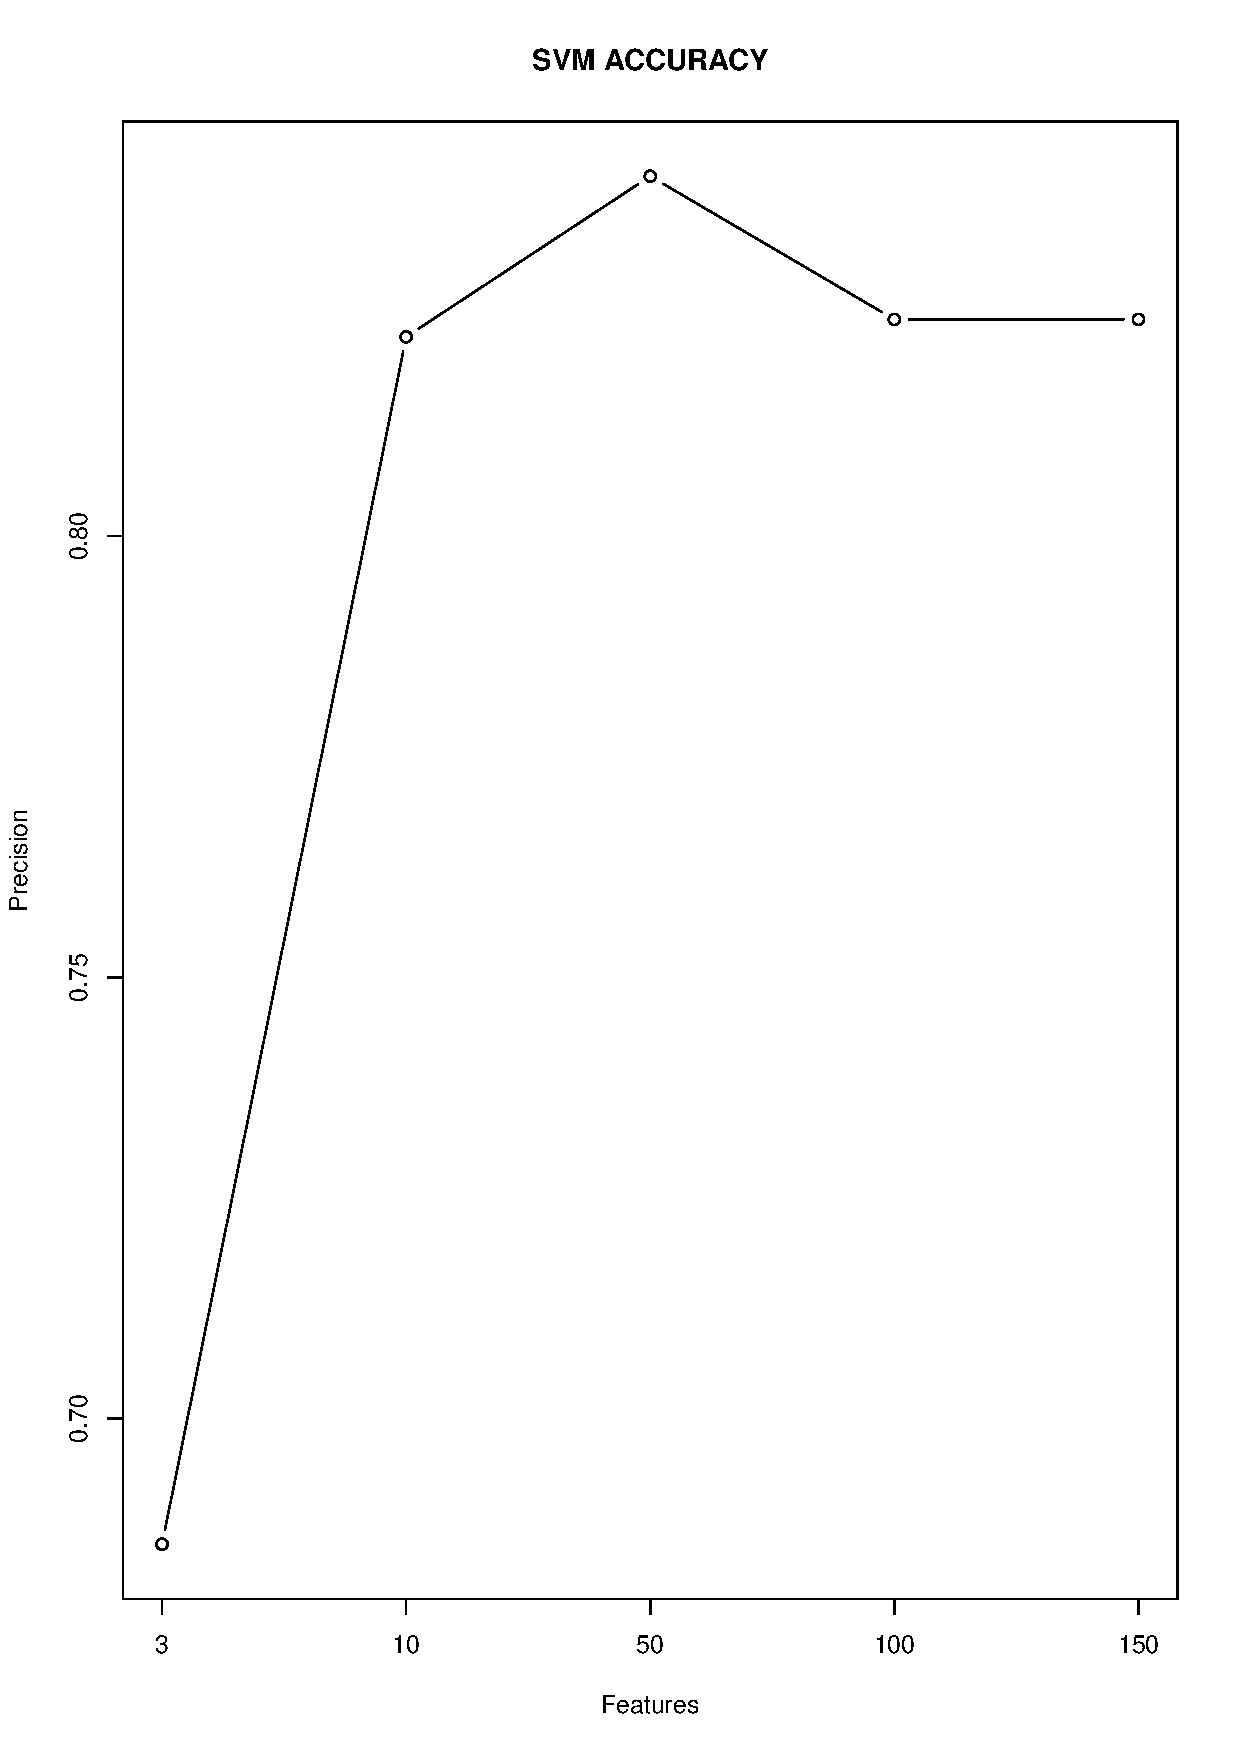
\includegraphics[scale=0.3]{../svm_accuracy_grayscale.pdf}
     }
     \subfloat{%
    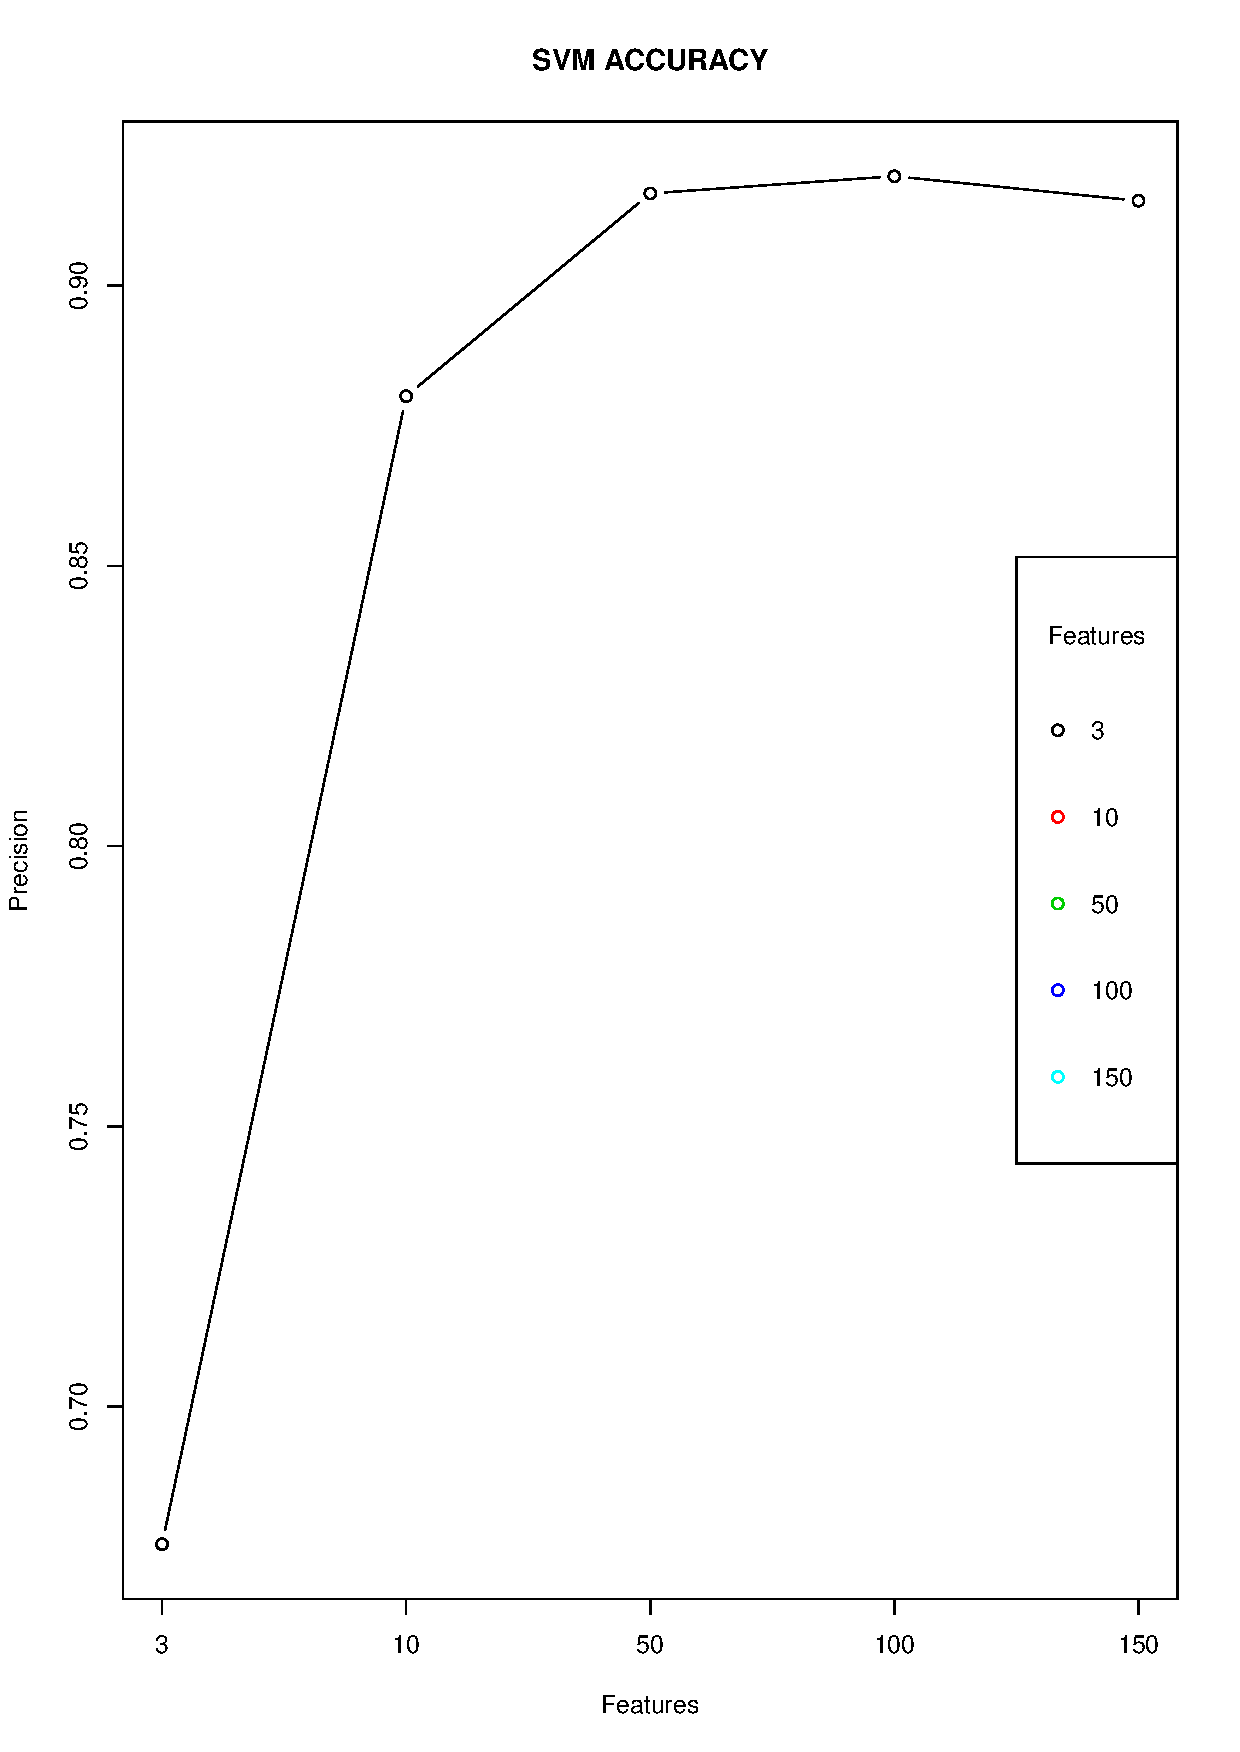
\includegraphics[scale=0.3]{../svm_accuracy_rgb.pdf}  
     }
     \centering
     \caption{Performance svm}
      \end{adjustwidth}
   \end{figure}
   
   
\begin{figure}[H]  
  \begin{adjustwidth}{-4cm}{-4cm}
     \subfloat{%
       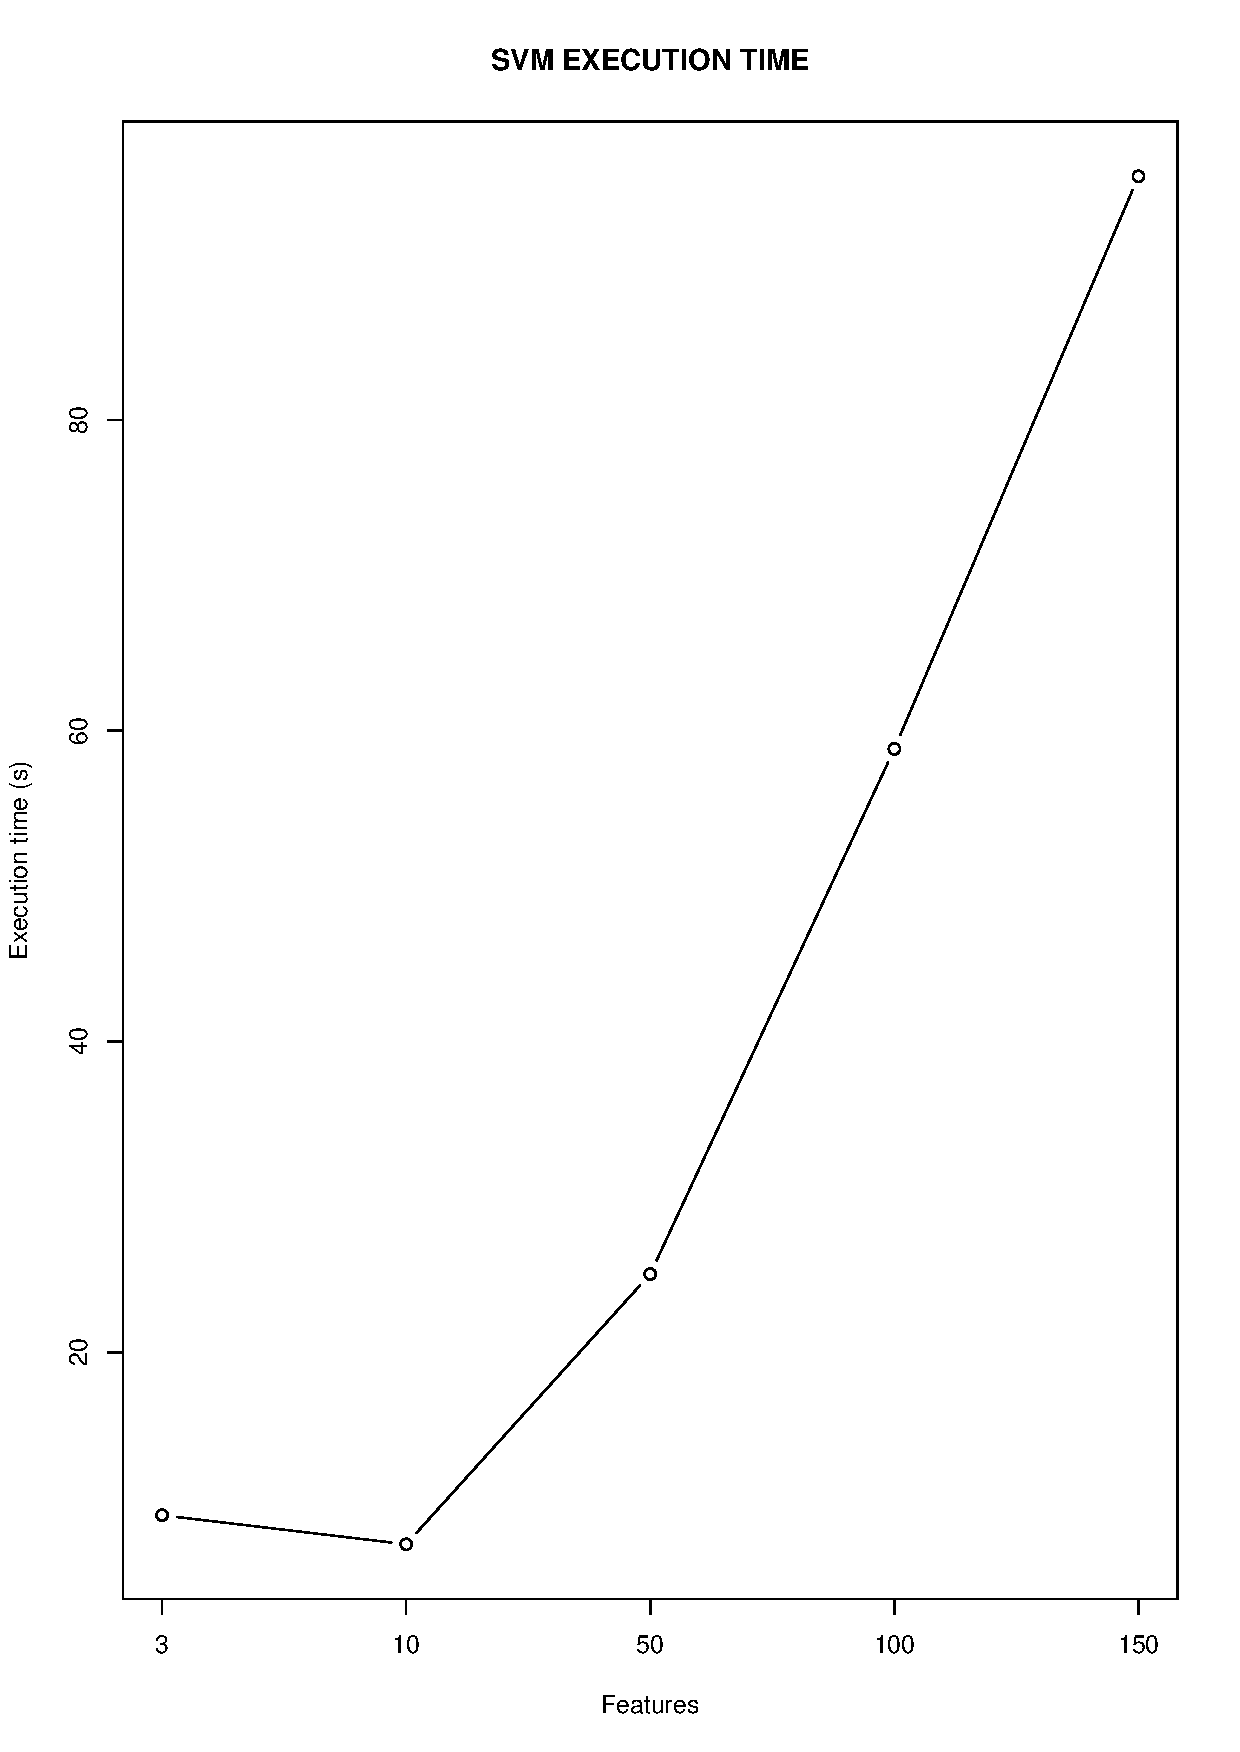
\includegraphics[scale=0.3]{../svm_time_grayscale.pdf}
     }
     \subfloat{%
    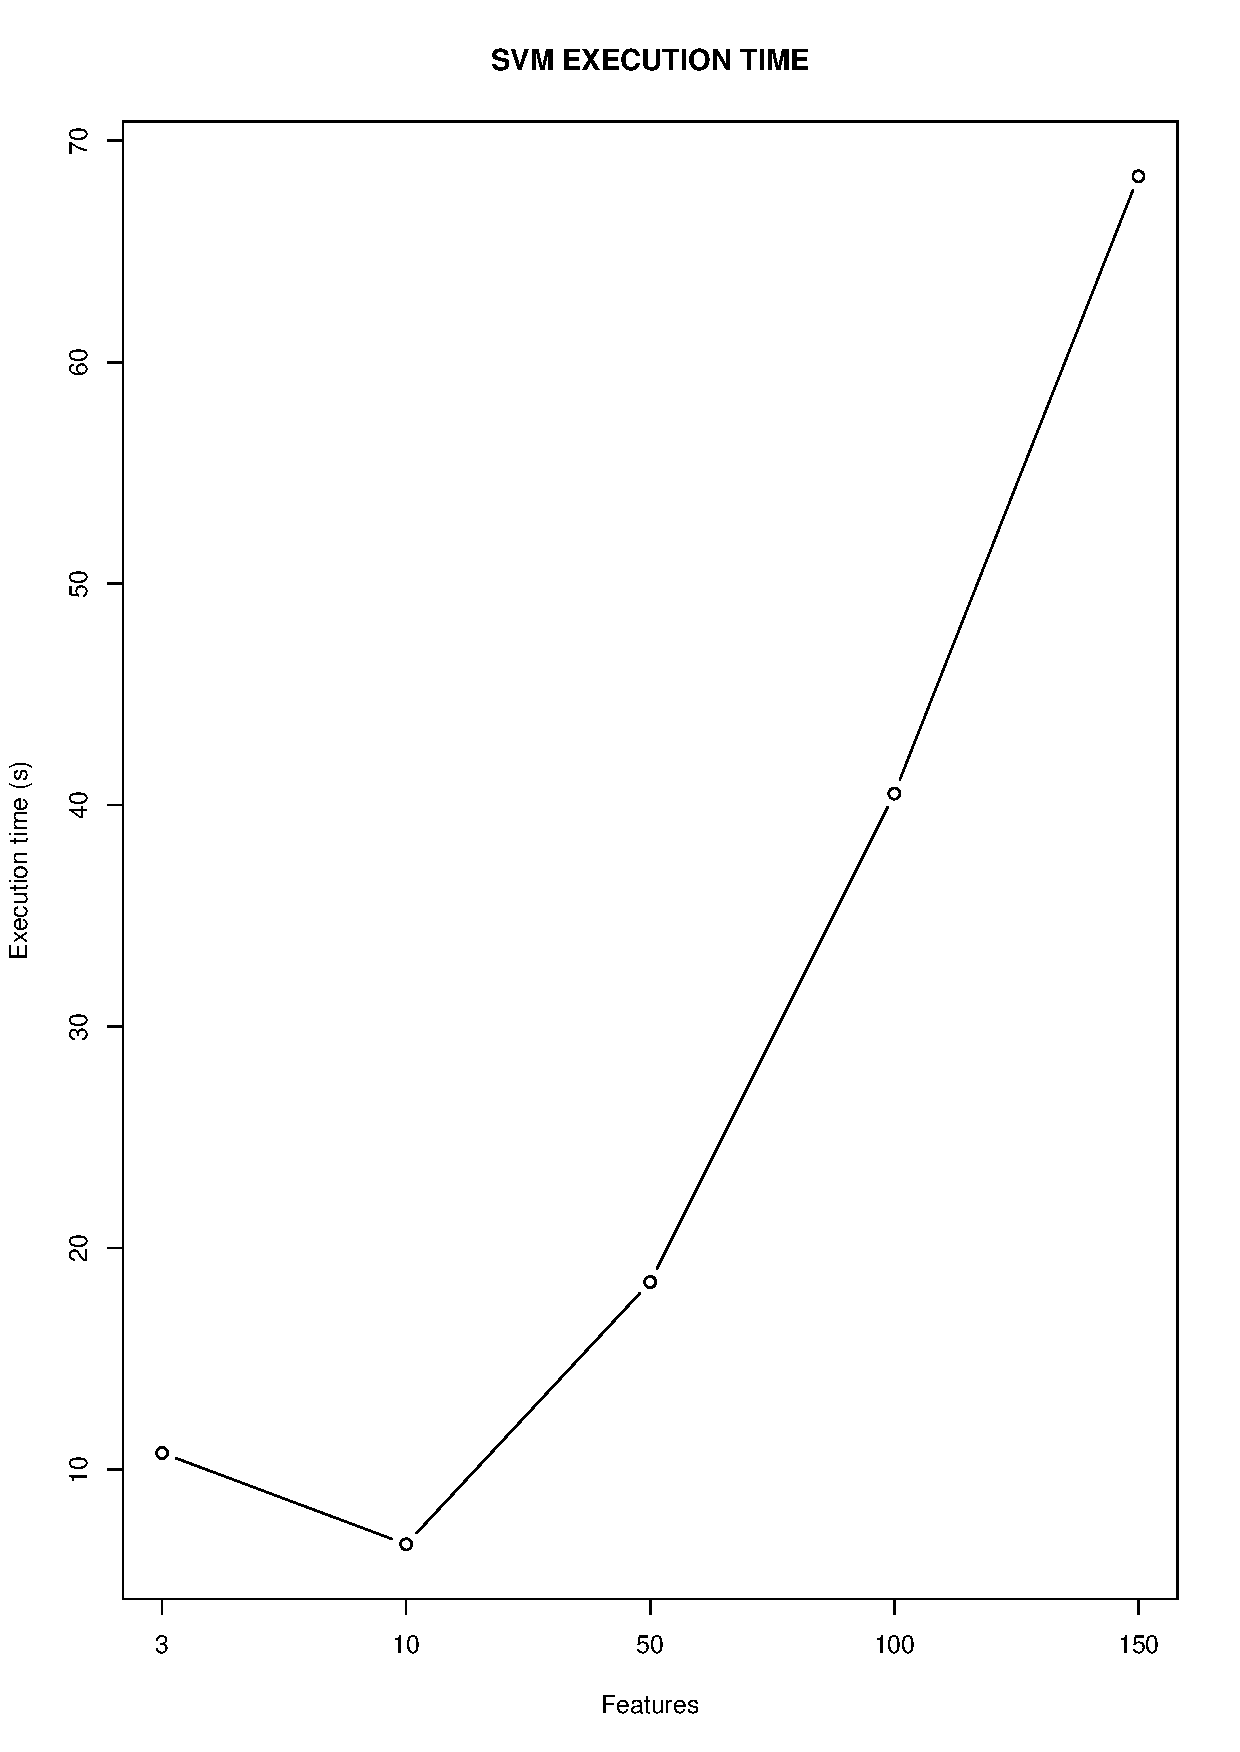
\includegraphics[scale=0.3]{../svm_time_rgb.pdf}  
     }
     \centering
     \caption{Execution time svm}
      \end{adjustwidth}
   \end{figure}


\newpage
\begin{thebibliography}{9}
\bibitem{dataset}
\textit{Horea Muresan, Mihai Oltean, Fruit recognition from images using deep learning, Acta Univ. Sapientiae, Informatica Vol. 10, Issue 1, pp. 26-42, 2018.}

\bibitem{review}
\textit{Khurram Hameed, Douglas Chai, Alexander Rassau, A comprehensive review of fruit and vegetable classification techniques. Image and Vision Computing 80 (2018) 22-44.}

\bibitem{grayscaleconversion}
\textit{Samuel Macedo, Givanio Melo, Judith Kelner, A comparative study of grayscale conversion techniques applied to SIFT descriptors, SBC Journal on Interactive Systems, volume 6, number 2, 2015.}

\bibitem{knnresults}
\textit{Sandeep Kumar, Zeeshan Khan, Anurag jain, A Review of Content Based Image Classification using Machine Learning Approach, International Journal of Advanced Computer Research (ISSN (print): 2249-7277 ISSN (online): 2277-7970) Volume-2 Number-3 Issue-5 September-2012}

\end{thebibliography} 
\end{document}


